\documentclass[../main.tex]{subfiles} 

\renewcommand{\imageSrc}{../images/}
\renewcommand{\codeSrc}{../code/}

\begin{document}
\chapter{Fault Tolerance}

\section{Fault Classification}
Faults can either be due to material failure or human failure. 
\begin{itemize}
	\item \textbf{Material Faults}
	\begin{itemize}
		\item Permament (broken optical fiber)
		\item Transient (cosmic ray changes value bit in memory)
		\item Internal Fault (overheating due to fan malfunction)
		\item Environment Fault (power failure with no UPS)
	\end{itemize}
	\item \textbf{Human Faults}
	\begin{itemize}
		\item Design Errors (analysis or programming error)
		\item Interaction Error (wrong action by user or wrong data received from sensor)
	\end{itemize}
\end{itemize}
Errors in data processing:
\begin{center}
\begin{tabular}{|c|c|c|}
\hline 
• & Data NOK & Data OK \\ 
\hline 
Data Rejected & • & Error 1 \\ 
\hline 
Faulty Result & Error 2 & Error 3 \\ 
\hline 
System Crach & Error 4 & Error 5 \\ 
\hline 
\end{tabular} 
\end{center}
Errirs 4 and 5 are \textbf{Fail Stop} errors. They're easy to detect because in case of a problem everything stops. Error 2 and 3 are more vicious, the system continues to work but not as intended. 
\section{Reliability Metrics}
Reliability is measured by looking at what happens to a set of similar items. With $N$ the amount of items:
\begin{itemize}
	\item $S(t)$ is the number of surviving items after time $t$.
	\item $F(t)$ is the number of faulty items after time $t$.
\end{itemize}
Now we can define the \textbf{reliability} of this kind of itmes as 
\[
R(t) = \frac{S(T)}{N}
\]
We define the \textbf{failure rate} as:
\[
\text{Failure Rate} = \frac{1}{S(t)} \frac{dF(t)}{dt}
\]
We define the \textbf{mean time between failures (MTBF)} as:
\[
\text{MTBF} = \int_0^{\infty} R(T) dt
\]
R is a dimensionless value representing time. The MTBF is the surface under the curve representing the evolution with respect to $R(t)$, which is the percentage of surviving items after $t$.
\begin{figure}[h!]
    \centering
    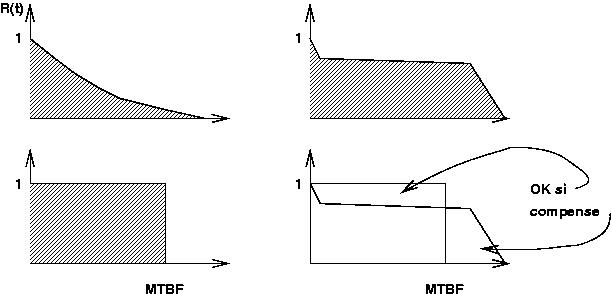
\includegraphics[width=0.8\textwidth]{\imageSrc/mtbf1.jpg}
    \caption{MTBF Illustration}
    \label{mtbf1}
\end{figure}
\\
Consider the two items on the right. After an initial drop corresponding to manufacturing defects R(t) stays nearly constant for a rather log time. This is the useful life time of the items. Extending the guarantee trough this time span is not expensive but has a psychological effect on clients. (this is why several manufacturers give long guarantees)
Later on, wear begins to show and the number of surviving items drops. This curve shows that the MTBF will often be before the end of the plateau. It is therefore a good measurement of the time an item can be expected to work.
\\\\
However, the MTBF cannot always be considered equal to the useful life of an item. For some devices, two values are published: the MTBF and the lifetime. In this case the computation of the MTBF is obtained by linear interpolation of R(t) at the beginning of the lifetime.

\begin{exmp}
An MTBF over 500.000 hours are given for hard disks along with a lifetime of 5 years. Knowing that a year includes 8760 hours, it means a MTBF of 57 years. In that case, the MTBF tells only that, after the time of early failures less that about 10\% of the disk might have a problem during their useful life. Disks intended for servers often have a guarantee equal to their lifetime.
\end{exmp}

Other useful metrics are the \textbf{availability} $A(t)$ and the \textbf{MTTR (Mean Time to Repair)}:
\[
A(t) = \frac{T_{\text{on}}}{T_{\text{on}} + T_{\text{off}}}
\]
\[
A(t) = \frac{T_{\text{on}}}{T_{\text{on}} + (N_{\text{faults}} \times \text{MTTR})}
\]
\[
N_{\text{faults}} = \frac{T_{text{ON}}}{\text{MTBF}}
\]
\[
A(t) = \frac{\text{MTBF}}{\text{MTBF} + \text{MTTR}}
\]
\section{Doubled Systems}
The purpose of doubled systems is to \textbf{minimize the MTTR}. There are multiple ways to implement doubled systems.

\subsection{Standby Redundancy}
With standby redundancy a spare system must be started. This might take up to 15 or 30 minutes before becoming fully operational. Improvements are possible to limit reconfiguration time. (= disconnecting equipment from one system and connecting it to another) Examples are shared peripherals between the main and spare system or the use of dual port peripherals.

\subsection{Active Redundancy}
The problem with active redundancy is threefold:
\begin{itemize}
	\item Decision to switch between main and spare
	\item Synchronization between main processor and spare processor
	\item Restart the processor that halted
\end{itemize}



\subsubsection{Basic Solution}
\begin{figure}[h!]
    \centering
    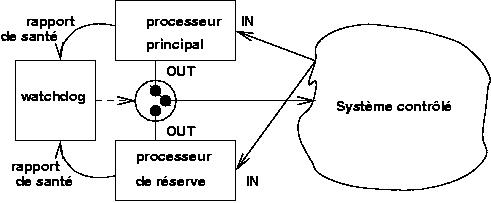
\includegraphics[width=0.8\textwidth]{\imageSrc/active_basic.jpg}
    \caption{Active Redundancy}
    \label{acre}
\end{figure}

A health report consists or a regular message indicating that the system is still alive, assuming the system is a \textbf{fail/stop system}. Al alternative might be a signature based on significant components of the system. This signature may be created at regular intervals or at each significant state change. Synchronization is handled by the events occurring at the controller system. A watchdog decides to switch to the spare processor. 
\\\\
A restart is handled by copying the state of the current main processor to the spare one. During this, the main processor might be stopped. If not, delicate techniques are used to synchronize distributed systems.
\\\\
It's important that the watchdogs doesn't fail! Only if it fails without disrupting the system's mission it is simple and robust.





\subsubsection{TANDEM Solution}

\section{Multiple Systems}

\end{document}